%%%%%%%%%%%%%%%%%%%%%%%%%%%%%%%%%%%%%%%%%%%%%%%%%%%
%% LaTeX book template                           %%
%% Author:  Amber Jain (http://amberj.devio.us/) %%
%% License: ISC license                          %%
%%%%%%%%%%%%%%%%%%%%%%%%%%%%%%%%%%%%%%%%%%%%%%%%%%%

\documentclass[a4paper,11pt]{book}
\usepackage[T1]{fontenc}
\usepackage[utf8]{inputenc}
\usepackage{lmodern}
%%%%%%%%%%%%%%%%%%%%%%%%%%%%%%%%%%%%%%%%%%%%%%%%%%%%%%%%%
% Source: http://en.wikibooks.org/wiki/LaTeX/Hyperlinks %
%%%%%%%%%%%%%%%%%%%%%%%%%%%%%%%%%%%%%%%%%%%%%%%%%%%%%%%%%
\usepackage{hyperref}
\usepackage{graphicx}
\usepackage[francais]{babel}
\usepackage{pdfpages}

%%%%%%%%%%%%%%%%%%%%%%%%%%%%%%%%%%%%%%%%%%%%%%%%%%%%%%%%%%%%%%%%%%%%%%%%%%%%%%%%
% 'dedication' environment: To add a dedication paragraph at the start of book %
% Source: http://www.tug.org/pipermail/texhax/2010-June/015184.html            %
%%%%%%%%%%%%%%%%%%%%%%%%%%%%%%%%%%%%%%%%%%%%%%%%%%%%%%%%%%%%%%%%%%%%%%%%%%%%%%%%
\newenvironment{dedication}
{
   \cleardoublepage
   \thispagestyle{empty}
   \vspace*{\stretch{1}}
   \hfill\begin{minipage}[t]{0.66\textwidth}
   \raggedright
}
{
   \end{minipage}
   \vspace*{\stretch{3}}
   \clearpage
}

%%%%%%%%%%%%%%%%%%%%%%%%%%%%%%%%%%%%%%%%%%%%%%%%
% Chapter quote at the start of chapter        %
% Source: http://tex.stackexchange.com/a/53380 %
%%%%%%%%%%%%%%%%%%%%%%%%%%%%%%%%%%%%%%%%%%%%%%%%
\makeatletter
\renewcommand{\@chapapp}{}% Not necessary...
\newenvironment{chapquote}[2][2em]
  {\setlength{\@tempdima}{#1}%
   \def\chapquote@author{#2}%
   \parshape 1 \@tempdima \dimexpr\textwidth-2\@tempdima\relax%
   \itshape}
  {\par\normalfont\hfill--\ \chapquote@author\hspace*{\@tempdima}\par\bigskip}
\makeatother


% Babel ``Sommaire'' à la place de ``table des matières''
\renewcommand{\contentsname}{Sommaire}


%%%%%%%%%%%%%%%%%%%%%%%%%%%%%%%%%%%%%%%%%%%%%%%%%%%
% First page of book which contains 'stuff' like: %
%  - Book title, subtitle                         %
%  - Book author name                             %
%%%%%%%%%%%%%%%%%%%%%%%%%%%%%%%%%%%%%%%%%%%%%%%%%%%

% Book's title and subtitle
\title{\Huge \textbf{Apprentissage dans les architectures cognitives}   \\ \huge contributions pour l'informatique et les neurosciences}
% Author
\author{\textsc{Emmanuel Daucé}}%\thanks{\url{www.example.com}}}


\begin{document}

\frontmatter
\maketitle

%%%%%%%%%%%%%%%%%%%%%%%%%%%%%%%%%%%%%%%%%%%%%%%%%%%%%%%%%%%%%%%
% Add a dedication paragraph to dedicate your book to someone %
%%%%%%%%%%%%%%%%%%%%%%%%%%%%%%%%%%%%%%%%%%%%%%%%%%%%%%%%%%%%%%%
\begin{dedication}
Dedicated to Calvin and Hobbes.
\end{dedication}

%%%%%%%%%%%%%%%%%%%%%%%%%%%%%%%%%%%%%%%%%%%%%%%%%%%%%%%%%%%%%%%%%%%%%%%%
% Auto-generated table of contents, list of figures and list of tables %
%%%%%%%%%%%%%%%%%%%%%%%%%%%%%%%%%%%%%%%%%%%%%%%%%%%%%%%%%%%%%%%%%%%%%%%%
\tableofcontents
\listoffigures
\listoftables

\mainmatter

\section*{Remerciements}
\begin{itemize}
\item A special word of thanks goes to Professor Don Knuth\footnote{\url{http://www-cs-faculty.stanford.edu/~uno/}} (for \TeX{}) and Leslie Lamport\footnote{\url{http://www.lamport.org/}} (for \LaTeX{}).
\item I'll also like to thank Gummi\footnote{\url{http://gummi.midnightcoding.org/}} developers and LaTeXila\footnote{\url{http://projects.gnome.org/latexila/}} development team for their awesome \LaTeX{} editors.
\item I'm deeply indebted my parents, colleagues and friends for their support and encouragement.
\end{itemize}
\mbox{}\\
%\mbox{}\\
\noindent Amber Jain \\
\noindent \url{http://amberj.devio.us/}

%%%%%%%%%%%%%%%%
% NEW CHAPTER! %
%%%%%%%%%%%%%%%%


%%%%%%%%%%%%%%%%%%%%%%%%%%%%%%%%%%%%%%%%%%%%%%%%%%%%%%%%%%%%%%%%%%%%%%%%%%%%%%%%%%%%%%%%%%%%%%%%%%%%%%%%%%%%%%%%%%%
%%%%%%%%%%%%%%%%%%%%%%%%%%%%%%%%%%%%%%%%%%%%%%%%%%%%%%%%%%%%%%%%%%%%%%%%%%%%%%%%%%%%%%%%%%%%%%%%%%%%%%%%%%%%%%%%%%%
%%%%%%%%%%%%%%%%%%%%%%%%%%%%%%%%%%%%%%%%%%%%%%%%%%%%%%%%%%%%%%%%%%%%%%%%%%%%%%%%%%%%%%%%%%%%%%%%%%%%%%%%%%%%%%%%%%%
%%%%%%%%%%%%%%%%%%%%%%%%%%%%%%%%%%%%%%%%%%%%%%%%%%%%%%%%%%%%%%%%%%%%%%%%%%%%%%%%%%%%%%%%%%%%%%%%%%%%%%%%%%%%%%%%%%%
%%%%%%%%%%%%%%%%%%%%%%%%%%%%%%%%%%%%%%%%%%%%%%%%%%%%%%%%%%%%%%%%%%%%%%%%%%%%%%%%%%%%%%%%%%%%%%%%%%%%%%%%%%%%%%%%%%%
%%%%%%%%%%%%%%%%%%%%%%%%%%%%%%%%%%%%%%%%%%%%%%%%%%%%%%%%%%%%%%%%%%%%%%%%%%%%%%%%%%%%%%%%%%%%%%%%%%%%%%%%%%%%%%%%%%%
\chapter{Introduction}
%%%%%%%%%%%%%%%%%%%%%%%%%%%%%%%%%%%%%%%%%%%%%%%%%%%%%%%%%%%%%%%%%%%%%%%%%%%%%%%%%%%%%%%%%%%%%%%%%%%%%%%%%%%%%%%%%%%
%%%%%%%%%%%%%%%%%%%%%%%%%%%%%%%%%%%%%%%%%%%%%%%%%%%%%%%%%%%%%%%%%%%%%%%%%%%%%%%%%%%%%%%%%%%%%%%%%%%%%%%%%%%%%%%%%%%
%%%%%%%%%%%%%%%%%%%%%%%%%%%%%%%%%%%%%%%%%%%%%%%%%%%%%%%%%%%%%%%%%%%%%%%%%%%%%%%%%%%%%%%%%%%%%%%%%%%%%%%%%%%%%%%%%%%
%%%%%%%%%%%%%%%%%%%%%%%%%%%%%%%%%%%%%%%%%%%%%%%%%%%%%%%%%%%%%%%%%%%%%%%%%%%%%%%%%%%%%%%%%%%%%%%%%%%%%%%%%%%%%%%%%%%
%%%%%%%%%%%%%%%%%%%%%%%%%%%%%%%%%%%%%%%%%%%%%%%%%%%%%%%%%%%%%%%%%%%%%%%%%%%%%%%%%%%%%%%%%%%%%%%%%%%%%%%%%%%%%%%%%%%
%%%%%%%%%%%%%%%%%%%%%%%%%%%%%%%%%%%%%%%%%%%%%%%%%%%%%%%%%%%%%%%%%%%%%%%%%%%%%%%%%%%%%%%%%%%%%%%%%%%%%%%%%%%%%%%%%%%



\begin{chapquote}{Author's name, \textit{Source of this quote}}
``This is a quote and I don't know who said this.''
\end{chapquote}

% le modèle de Hopfield
% Qu'est-ce que le chaos?

% Qu'est-ce qu'un système apprenant



% Architectures de contrôle. Point de vue de la robotique. Automates embarqués. 

Quelle est la question?


% Philo
Créer du neuf à partir de rien.
Qu'est-ce que la nouveauté?
D'où vient l'information?

Potentialité et émergence. Notion d'historique. Constructivisme.
% Importance de l'activité intrinsèque
% Activité centrale flutuante, émergence, historique
% couplage sans fonction (corps sans organe)
% triptique : corps- société- organe (à différents niveaux) - organisme = société des organes
% analogie eonomique : composants - emploi - produit (composé)

% Ce que j'ai fait, quelles sont mes questions?

Les enjeux :

- Substrat apprenant (universel). 










%%%%%%%%%%%%%%%%%%%%%%%%%%%%%%%%%%%%%%%%%%%%%%%%%%%%%%%%%%%%%%%%%%%%%%%%%%%%%%%%%%%%%%%%%%%%%%%%%%%%%%%%%%%%%%%%%%%
%%%%%%%%%%%%%%%%%%%%%%%%%%%%%%%%%%%%%%%%%%%%%%%%%%%%%%%%%%%%%%%%%%%%%%%%%%%%%%%%%%%%%%%%%%%%%%%%%%%%%%%%%%%%%%%%%%%
%%%%%%%%%%%%%%%%%%%%%%%%%%%%%%%%%%%%%%%%%%%%%%%%%%%%%%%%%%%%%%%%%%%%%%%%%%%%%%%%%%%%%%%%%%%%%%%%%%%%%%%%%%%%%%%%%%%
%%%%%%%%%%%%%%%%%%%%%%%%%%%%%%%%%%%%%%%%%%%%%%%%%%%%%%%%%%%%%%%%%%%%%%%%%%%%%%%%%%%%%%%%%%%%%%%%%%%%%%%%%%%%%%%%%%%
%%%%%%%%%%%%%%%%%%%%%%%%%%%%%%%%%%%%%%%%%%%%%%%%%%%%%%%%%%%%%%%%%%%%%%%%%%%%%%%%%%%%%%%%%%%%%%%%%%%%%%%%%%%%%%%%%%%
%%%%%%%%%%%%%%%%%%%%%%%%%%%%%%%%%%%%%%%%%%%%%%%%%%%%%%%%%%%%%%%%%%%%%%%%%%%%%%%%%%%%%%%%%%%%%%%%%%%%%%%%%%%%%%%%%%%
\chapter{Architectures cognitives}
%%%%%%%%%%%%%%%%%%%%%%%%%%%%%%%%%%%%%%%%%%%%%%%%%%%%%%%%%%%%%%%%%%%%%%%%%%%%%%%%%%%%%%%%%%%%%%%%%%%%%%%%%%%%%%%%%%%
%%%%%%%%%%%%%%%%%%%%%%%%%%%%%%%%%%%%%%%%%%%%%%%%%%%%%%%%%%%%%%%%%%%%%%%%%%%%%%%%%%%%%%%%%%%%%%%%%%%%%%%%%%%%%%%%%%%
%%%%%%%%%%%%%%%%%%%%%%%%%%%%%%%%%%%%%%%%%%%%%%%%%%%%%%%%%%%%%%%%%%%%%%%%%%%%%%%%%%%%%%%%%%%%%%%%%%%%%%%%%%%%%%%%%%%
%%%%%%%%%%%%%%%%%%%%%%%%%%%%%%%%%%%%%%%%%%%%%%%%%%%%%%%%%%%%%%%%%%%%%%%%%%%%%%%%%%%%%%%%%%%%%%%%%%%%%%%%%%%%%%%%%%%
%%%%%%%%%%%%%%%%%%%%%%%%%%%%%%%%%%%%%%%%%%%%%%%%%%%%%%%%%%%%%%%%%%%%%%%%%%%%%%%%%%%%%%%%%%%%%%%%%%%%%%%%%%%%%%%%%%%
%%%%%%%%%%%%%%%%%%%%%%%%%%%%%%%%%%%%%%%%%%%%%%%%%%%%%%%%%%%%%%%%%%%%%%%%%%%%%%%%%%%%%%%%%%%%%%%%%%%%%%%%%%%%%%%%%%%


\section{Problématique}

Une architectures cognitives est un dispositif logiciel dont le but est de permettre à un appareil 
(disposant de capteurs et d'actuateurs) d'interagir de façon ``intelligente'' avec son environnement. 
Le concept de comportement intelligent reste bien sûr assez flou.
On assimilera ici  dispositif logiciel et contrôleur. 
On parlera de signal d'entrée pour qualifier les données analogiques ou digitales à traiter.     
On parlera de commande pour qualifier la réponse (analogique ou digitale) produite par le dispositif.

Ce problème d'une définition opérationnelle de l'intelligence a été posé au sortir de la deuxième guerre mondiale. 
Il s'agissait de construire un programme de recherche, une feuille de route détaillant les étapes nécessaires 
et suffisantes pour construire un dispositif artificiel intelligent.

A un niveau très général, le but est de produire un dispositif dont les réponses s'apparenteraient dans la forme et dans le contenu à celles d'un être humain,
tout en reposant sur des opérations élémentaires issues d'un traitement mécanico-logique de l'information.
Cet objectif est exprimé de façon claire par le test de Turing [REF]: un dispositif intelligent doit être capable 
de communiquer avec un être humain de manière naturelle, c'est à dire qu'il soit impossible pour l'opérateur humain,
en l'absence de contact visuel, 
de savoir s'il s'adresse à une machine ou à un être humain.

Dans le domaine de la psychologie, l'émergence des sciences cognitives est venu en réaction au behaviorisme.
A l'origine, il s'agit de contester la description de l'activité du sujet comme simple courroie de transmission 
(un tableau de branchement) entre des stimuli et des réponses. Par opposition, il s'agit de décrire (proposer un modèle)
du sujet en tant qu'acteur. Notion d'agentivité (imputabilité de l'action).
%Toujours à ce niveau très général, une des notions clés de l'intelligence artificielle naissante est la notion d'agentivité, %autrement dit
%l'imputabilité de l'action. 
Un dispositif logico-mécanique pourrait être dit intelligent s'il était considéré comme responsable de ses actes, 
celui auquel on pourrait imputer les actions produites. 

Ces deux notions (test de Turing, agentivité) ne sont pas opérationnelles. Elles permettent de tracer des frontières par exclusion. Un dispositif logiciel
n'est pas vu comme intelligent s'il ne passe pas le test de Turing, 
ou si on ne peut pas lui imputer les réponses qu'il a produites.
Elles sont néanmoins toutes deux imparfaites, puisque reposant in fine sur la subjectivité de l'observateur.
Différents contre-exemples peuvent d'ailleurs être trouvés dans lesquels des dispositifs
logico-mécaniques (machines) produisant des illusions, autrement dit sont tels que l'opérateur humain tend à 
leur attribuer des intentions qui n'y sont pas [BRAITENBERG]. Attribuer des intentions est un biais perceptif humain.

Une approche plus opérationnelle consiste à décrire (lister) les compétences attendues de la part du logiciel.
Si on se réfère aux conceptions courantes de l'intelligence, 
il s'agit de décrire, modéliser mathématiquement et reproduire mécaniquement le sujet cognitif, capable de:
\begin{enumerate}
\item raisonner (agglomérer différents faits pour déduire des faits nouveaux - et/ou des réponses) - l'acuité (perspicacité) du raisonnement, 
c'est à dire la capacité à établir des faits nouveaux à partir de faisceaux d'indices (par déduction) - {\color{red} compatible paradigme behavioriste}
\item se rappeler (prendre en considération certains faits anciens (acquis) en plus des faits imédiatement disponibles) - la memoire est liée à la notion d'``etat interne''. Croyance, Prior.
\item apprendre (intégrer de nouveaux faits, remettre en cause certains faits acquis) - {\color{red} compatible paradigme behavioriste}.
\item planifier et faire des choix, c'est à dire évaluer les bénéfices et les pertes attendus des actions ou des réponses produites.
\item etc.
\end{enumerate}

Dans ce cas (définition extensive de l'intelligence), plusieurs problèmes se posent. Il est (1) difficile de séparer les différents items et (2) difficile de fermer la liste. Selon le point de vue que l'on adopte, raisonner (établir de faits) 
peut s'apparenter à décider (établir des actes). La mémoire, c'est à la fois se rappeler et intégrer des faits nouveaux.
Le raisonnement ne peut s'établir sur la base des observations immédiates, il doit intégrer des faits mémorisés etc. 
Chacune de ces capacités (raisonner, stocker en mémoire, planifier,...) peut être implémentée
dans certains contextes sans que le comportement du logiciel soit considéré comme intelligent au sens plein. 
On pensera par exemple aux logiciels d'échec ou de go qui tendent à atteindre les capacités des experts humains,
aux logiciels d'aide à la décision, aux pilotes automatiques, ... 
Enfin, il est difficile d'exclure de la liste certaines capacités comme l'intelligence pratique (sens
pratique, capacités opérationnelles, répertoire de comportements, agilité...)
ou encore l'intelligence émotionnelle, intelligence verbale, etc... qui ont reçu chacune des tentatives de définition. 

Cette approche (lister des compétences) est une approche typiquement réductionniste, consistant à découper un problème
en sous-problèmes pour mieux les analyser et les résoudre.
Malgré les nombreuses tentatives, il s'est de plus avéré que l'assemblage de briques
logicielles présentant des compétences élémentaires aboutissait rarement à un système efficace. 
Dans le cas des système experts par exemple, le pur raisonnement sur les faits élémentaires aboutit rarement 
à une réponse réellement exploitable. Les logiciels de traduction ou correction automatiques les plus efficaces 
reposent sur les régularité statistiques, pas sur l'analyse de la structure de la phrase. 

Chaque item : calcul - mémoire - décision est un problème en soi, 
sujet à débat et controverse.
Chaque item semble aussi peu opérationnel que le terme plus englobant d'intelligence.

Problème de la compétence universelle (ou et quand appliquer la bonne méthode). 
Choix de la méthode. 
Versatilité.
Compétences multiples (séquentielle) vs. compétence intégrée (toutes les compétences en même temps).
Difficulté à traiter des environnements complexes. 
Le problème de la compétence globale a tendance à dégénérer en problème
du choix (de la bonne brique logicielle). Exemple des robots-jouets. Que faire dans une situation
qui n'a pas été prévue par le concepteur? Augmentation de la complexité. 
Chaque brique résout un problème spécifique. Tendance à l'``usine à gaz''.

ref : general proble solver (Simon - Newell).
Architecture SOAR (voir Wikipedia)

Le problème devient : l'intelligence, c'est atteindre un comportement adapté 
qui n'avat pas été prévu au départ par le concepteur. Capacité ``créative''. Capacité à faire face,
adaptivité.
Déplacement du problème : qu'est-ce qu'un comportement adapté?
 
Par opposition à l'approche réductionniste, nous 
considérerons dans la suite de ce document l'approche dite constructiviste, ou développementale, 
consistant à établir des règles de construction plutôt que des prescriptions.
On parle également de démarche ``bottom-up''.
Principe fondateur.

Problème : plusieurs principes fondateurs en concurrence. 

Dans ce cas, plusieurs ``bases'' possibles : (1) logico-symbolique et dualité donnée-programme. Traitement (calculateur) ``digital''.
Historiquement la plus ancienne. Possibilité d'écrire 
dans le programme. Principalement notion de méta programme (programme constructeur de programme). 
Métaphore de l'ordinateur. Un ordinateur est doué de capacités de calcul, de mémoire et d'actuateurs.
L'IA revient ici à définir/décrire le méta programme. 
(2) Mécanique. Principe de la régulation (cybernétique). Action et imputabilité. Traitement (calculateur) ``analogique''. 
Importance des interactions mécaniques (approche située). Variables de contrôle. 
Comportement d'écart/retour à l'équilibre. Mais : calcul? mémoire? ODE. 
(3) Traitement du signal + neuro-inspiré. Calcul distribué. Filtre. Auto-organisation. Population. Emergence. Attracteur. EDP? 

De façon intéressante, on retrouve dans les 3 cas un raisonnement ``qui se mord la queue''. 

Les fondateurs des sciences cognitives ont placé très tôt la question de l'apprentissage  au coeur de leur problématique 
(qu'est-ce qu'une machine intelligente - cf. Turing)

Question de l'autonomie. Augmentation de l'autonomie des programmes au cours du temps. Décharge cognitive mais pas 
d'autonomie véritable. Déplacement de la définition de l'intelligence (concept insaisissable).

Deux approches/réponses se dessinent dès l'origine :  
\begin{itemize}
 \item traitement symbolique
 \item traitement analogique
\end{itemize}
L'enjeu principal est celui d'un côté du traitement analogique et de l'autre le traitement symbolique. Du point de vue des sciences cognitives naissantes, c'est le traitement
symbolique qui gagne dans un premier temps.

Dans ces deux formalismes, la question de l'apprentissage a eu tendance à progressivement se marginaliser au profit (1) du traitement logique des symboles et de modèles
 descriptifs du langage (grammaires génératives) et (2) l'ingéniérie et la conception de systèmes d'asservissement de plus en plus complexes et/ou psychologie et constructivisme (Palo Alto)

A l'inverse, la question de l'apprentissage est restée présente dans le domaine des sciences de l'information et l'informatique naissante. 
La question de l'apprentissage  devient la question de construire des programmes (des automates) capables de se modifier, de s'amender pour mieux répondre aux sollicitations
de l'environnement. Cette question étant posée (comment modifier le programme sans intervention humaine), le formalisme des réseaux de neurones et du calcul distribué 
s'est révélé le plus apte à traiter la question --> le perceptron. 

\paragraph{Intérêt}

\begin{itemize}
 \item déplacement de la charge cognitive (mais augmente la dépendance de l'homme au dispositif)
 \item personnalisation - accès à l'information (mais risque de ``flicage'' - problème de confidentialité)
 \item véhicules autonomes
 \item maison/environnement intelligent
\end{itemize}


Une architecture cognitive est alors une proposition de réalisation logicielle de ce cahier des charges (un logiciel capable de raisonner, se souvenir et faire des choix).
On distingue classiquement 3 approches pour la réalisation de telles architectures. 
\begin{enumerate}
 \item approche logico-mathématique 
 \item approche mécanique
 \item approche traitement du signal
\end{enumerate}

On regarde dans le détail ces trois approches avec un focus particulier sur l'apprentissage et l'autonomie. 

\subsection{Approche logico-mathématique}

(CALCUL - CALCULABILITE)

Focus sur le langage et le traitement syntaxique - l'intelligence est manipulation de symboles - structuralisme - arbitraire du signe - tout est langage

Machine à états.  Manipulaton de symboles. Connaissances et croyances. L'essentiel de l'effort a porté sur le traitement symbolique de l'information: 
la mémoire - la perception - les grammaires génératives - la logique formelle. Ces modèles cognitifs se focalisent sur la notion de croyance, c'est à dire 
d'état interne qui conditionne la réponse. (x, etat => y, LUT). Par extension, etat = connaissance, prior. Le prior peut biaiser la reponse. 
Mais (péché) traitement symbolique = examen séquentiel des faits. Peu de prise en compte de l'extension spatiale.


\subsection{Approche mécanique}

(FEEDBACK)

Systèmes dynamiques. (MECANIQUE) Notion d'équilibre dynamique (forces opposantes). Homéostasie. Wiener. Architectures de contrôle basées sur des variables de contrôle. Notion d'écart/erreur.  
L'agentivité se caractérise par le maintien actif de variables de contrôle à l'intérieur d'un certain intervalle. + Palo Alto. 
La contestation du paradigme behavioriste passe par la notion de contrôle ``reactif'' et d'ecart à l'equilibre. Notion de contrôleur/fonction de contrôle. On ne considère pas des 
``mappings'' stimulus-réponse discrets (x => y, LUT) mais des couples $(x_0,k)$ avec $y = k (x - x_0) $.    
Modèle inverse.  Architecture de contrôle et autonomie.

La plupart des logiciels et les
applications utilisées dans la vie courante sont considérés comme ``non intelligents''. Ce sont des dispostifs ``commandés'', c'est à dire obéissant aux consignes 
et dont la réponse ne varie pas au cours du temps, ou d'une utilisation à l'autre. Ce comportement (conformité de la réponse à la consigne) est souhaitable dans la plupart
des cas. 
Toujours dans le domaine de la vie courante, est ``non intelligent'' tout ce qui est prévisible, ce que l'on peut manipuler, exploiter.

Il ressort : est intelligent ce qui n'est pas prévisible, 


\subsection{Approche traitement du signal}

(OPTIMISATION)


% L'émergence des neurosciences computationnelles
L'inspiration naturelle. Au cours de l'histoire des sciences cognitives, plusieurs rapprochements ont eu lieu avec les sciences du vivant et les neurosciences:

- Années 40 : modèle McCullogh et Pitts, plasticité de Hebb. Assemblée neuronale. Notion de représentation distribuée?

- Années 60 : modèles de la vision, le perceptron. Implémentation. Filtre. Classifieur. Feed-forward.

- Années 80 : modèle de Hopfield. Physique statistique. 


Analogie biologique. Calcul distribué. Le perceptron est à la base un modèle de la perception visuelle. Le perceptron apporte de nombreux concepts nouveaux qui 
vont s'avérer féconds pour les sciences cognitives.   

D'un côté, il appartient à double titre à une famille des modèles ``behavioristes''. Le perceptron est bien un tableau de branchement.
Sa règle de mise à jour repose sur des causalités stimulus-réponse.  
De l'autre, il introduit les concepts de filtres, de pattern matching et de calcul distribué, avec un fonctionnement qui diffère à  la fois 
du traitement logico-symbolique et du contrôle intensif/analogique.

Si le perceptron constitue un pas en arrière par rapport à certains prémisses des sciences cognitives (agentivité), il constitue néanmoins un pas en avant important 
puisqu'il produit un modèle généralisable de calcul distribué, c'est à dire qu'il propose une première implémentation décentralisée de l'apprentissage et de la plasticité.
On sort des approches logico-symboliques avec la prise en compte de l'organisation (extension) spatiale des stimuli.
(THERMODYNAMIQUE - PHYSIQUE STAT - TRAITEMENT DU SIGNAL - CHAMP)

Il s'agit d'un modèle nouveau qui ne tire ses prémisses ni du calcul symbolique centralisé (machine de Turing), ni de la théorie des systèmes dynamiques, mais
plutot de l'observation de l'organisation à l'oeuvre dans les premières couches du traitement visuel. L'apprentissage est bien guidé par la 
correction d'erreurs, mais agit dans l'espace des paramètres. 

Voir aussi Hubel et Wiesel.

A différentes époques, les neurosciences se sont mises à l'agenda des sciences cognitives. C'est en puisant dans les connaisances biologiques
de leur époque que les sciences cognitives ont pu se renouveler.

Réseaux de neurones et boite noire.
Qui dit décentralisé dit boite noire difficile à interpréter...

L'apprentissage automatique s'est développé/autonomisé et se ramène souvent à des statistiques descriptives...
Dans ce cadre, un système apprenant est une machine à entrées-sorties, une fonction paramétrique, dont les paralètres on au choix : 
un degré de vraisemblance élevé, maximisent la séparation des données, ...
l'apprentissage devient un des branches de l'optimisation mathématique.


la théorie de l'information : caractériser le caractère informatif (ou non) d'un message par son degré de prédictabilité. Problème : les deux extrêmes (information nulle,
information maximale) sont inintéressants...
\--- Transmission de l'information \--- Emetteur et récepteur \--- débit. 

\section{Questions ouvertes}

\paragraph{Autonomisation des questions}

- question du langage

- question de l'apprentissage

- question du contrôle

- question du calcul

- etc...


\paragraph{Problèmes de consistance}

D'un côté (calculabilité). Le programme qui interprète des programmes. Dualité donnée / programme. Récursivité.  

Feedback négatif. Réponse soumise à l'entrée qui est soumise à la réponse.

Récurrence. Hystérèse.


EM


\paragraph{La question (le problème) de l'autonomie}

Le ``noeud'' du problème. Imputabilité.
Les points 1, 2 et 3 peuvent être réalisés sans imputabilité. Seul 4 (choix) a des 

Dans le langage courant, on entend par ``intelligence'' la capacité à agir de façon appropriée en différentes circonstances, autrement dit de produire
les réponses qui sont les plus à même de produire un bénéfice à l'agent 

Une première manière est de définir un dispositif cognitif par opposition à un dispositif ``commandé'', c'est à dire
capable de développer des comportements intelligents de façon autonome.


\paragraph{Neurosciences computationnelles}











%%%%%%%%%%%%%%%%%%%%%%%%%%%%%%%%%%%%%%%%%%%%%%%%%%%%%%%%%%%%%%%%%%%%%%%%%%%%%%%%%%%%%%%%%%%%%%%%%%%%%%%%%%%%%%%%%%%
%%%%%%%%%%%%%%%%%%%%%%%%%%%%%%%%%%%%%%%%%%%%%%%%%%%%%%%%%%%%%%%%%%%%%%%%%%%%%%%%%%%%%%%%%%%%%%%%%%%%%%%%%%%%%%%%%%%
%%%%%%%%%%%%%%%%%%%%%%%%%%%%%%%%%%%%%%%%%%%%%%%%%%%%%%%%%%%%%%%%%%%%%%%%%%%%%%%%%%%%%%%%%%%%%%%%%%%%%%%%%%%%%%%%%%%
%%%%%%%%%%%%%%%%%%%%%%%%%%%%%%%%%%%%%%%%%%%%%%%%%%%%%%%%%%%%%%%%%%%%%%%%%%%%%%%%%%%%%%%%%%%%%%%%%%%%%%%%%%%%%%%%%%%
%%%%%%%%%%%%%%%%%%%%%%%%%%%%%%%%%%%%%%%%%%%%%%%%%%%%%%%%%%%%%%%%%%%%%%%%%%%%%%%%%%%%%%%%%%%%%%%%%%%%%%%%%%%%%%%%%%%
%%%%%%%%%%%%%%%%%%%%%%%%%%%%%%%%%%%%%%%%%%%%%%%%%%%%%%%%%%%%%%%%%%%%%%%%%%%%%%%%%%%%%%%%%%%%%%%%%%%%%%%%%%%%%%%%%%%
\chapter{Parcours}
%%%%%%%%%%%%%%%%%%%%%%%%%%%%%%%%%%%%%%%%%%%%%%%%%%%%%%%%%%%%%%%%%%%%%%%%%%%%%%%%%%%%%%%%%%%%%%%%%%%%%%%%%%%%%%%%%%%
%%%%%%%%%%%%%%%%%%%%%%%%%%%%%%%%%%%%%%%%%%%%%%%%%%%%%%%%%%%%%%%%%%%%%%%%%%%%%%%%%%%%%%%%%%%%%%%%%%%%%%%%%%%%%%%%%%%
%%%%%%%%%%%%%%%%%%%%%%%%%%%%%%%%%%%%%%%%%%%%%%%%%%%%%%%%%%%%%%%%%%%%%%%%%%%%%%%%%%%%%%%%%%%%%%%%%%%%%%%%%%%%%%%%%%%
%%%%%%%%%%%%%%%%%%%%%%%%%%%%%%%%%%%%%%%%%%%%%%%%%%%%%%%%%%%%%%%%%%%%%%%%%%%%%%%%%%%%%%%%%%%%%%%%%%%%%%%%%%%%%%%%%%%
%%%%%%%%%%%%%%%%%%%%%%%%%%%%%%%%%%%%%%%%%%%%%%%%%%%%%%%%%%%%%%%%%%%%%%%%%%%%%%%%%%%%%%%%%%%%%%%%%%%%%%%%%%%%%%%%%%%
%%%%%%%%%%%%%%%%%%%%%%%%%%%%%%%%%%%%%%%%%%%%%%%%%%%%%%%%%%%%%%%%%%%%%%%%%%%%%%%%%%%%%%%%%%%%%%%%%%%%%%%%%%%%%%%%%%%











%Je propose dans cette partie de parcourire certains de mes travaux passés en essayant de proposer un éclairage/dégager une cohérence.

Un cadre unique pour l'apprentissage et la plasticité. La difficulté consiste à éclairer les méthodes de machine learning à partir de concepts issus des sciences cognitives. 
Essayer de construire un cadre conceptuel (ou de réexaminer des cadres conceptuels existants mais non explicités). 

Aller au delà des modèles actuels de l'apprentissage (essentiellement behavioristes) en reprenant toute la structure conceptuelle de l'apprentissage. 

D'un côté, le point de vue des sciences cognitives :
Agent incarné. Corps. Extension (du corps, du territoire) limitée. Ressources (computationnelles) limitées. 
Déplacement du corps et emploi du corps visant le retour à l'équilibre (dominé par des variables de type contrôle des apports énergétiques. 
Vient ensuite recherche d'abri, recherche de partenaires, etc...). 
Autonomie.

De l'autre, du point de vue du machine learning : extraterritorialité des données (peu de limite spatiale, ou absence d'extension spatiale). 
Ressources computationnelles distribuées (non localisées). Hétéronomie. L'accès aux ressources n'est pas un enjeu (dépend d'un agent extérieur).


En particulier : la notion d'expressivité du substrat est prometteuse. En particulier on pourra distinguer expressivité discrète (argmax discret) et expressivité continue (neural field).


- Substrat. Des ressources limitées (nombre de neurones N, pas de recrutement). Expressivité du substrat (discret/réel, dimension, richesse du comportement intrinsèque).  
(exemple de substrat à expressivité limitée : carte de Kohonen, réseau de Hopfield). (ART ajoute le recrutement).  Clustering.
L'universalité implique la mise en oeuvre de ressources indépendamment de la tâche (task-independent device). Le substrat doit au mieux exploiter ses ressources. 
A rappeler également : les niveaux de Marr : du substrat au modèle.
{\bf computation/traitement du signal basé sur la pattern matching (filtres) et non sur un traitement intensif/analogique (architectures de contrôle). Glissement de l'espace des actions 
à l'espace des paramètres}

- Potentialité et instanciation. Réservoir. Emergence = instanciation. Irréversibilité (historique). Sculpture du vivant. Réduction d'incertitude. Plasticité, STDP, Hebb...

- Fluctuation. Bruit - activité fluctuante. Activité intrinsèque. Activité de base. Création d'information. Capture. (Exemples de capture : le modèle acteur-critique, le réservoir computing).
Notion d'activité centrale fluctuante. Le chaos. Le bruit comme élément générateur, source de nouveauté.
L'activité intrinsèque n'est pas uniquement feed-forward (traitement du signal), lateral (inference) ou feedback (rappel). 
Il faut considérer la fluctuation imprévue et la création d'information. 
L'exploration apparait nécessaire dans les environements complexes : lorsque l'espace des tâches est complexe. Periode de jeu chez les mammifères. 
{\bf Fonction des fluctations = capture de nouveaux couplages dans un environnement complexe}

- Perception et non-sens. Pattern matching. UP/DOWN states. Ecart au modèle (Bayesian surprise). Predictive coding.
Activité de base. Reconnaissance par franchissement d'un seuil (``vigilance''). Distinction  entre connu et non-perçu (non-sens).
Modèles de la perception. Freeman.

- Engagement et action. Commande. Architectures de contrôle. Espace des tâches. Couplages corps-environnement (Friston). Organisme transitoire (Société des organes). 

- Variables de contrôle. Equilibre dynamique. Homeostasie. Emploi et Couplage sans emploi. Répertoire (dictionnaire?) d'emplois. 

- Séquence. Causalité

- Apprendre et oublier. Online learning. 


Question : atteint-on une limite des rapprochements entre sciences cognitives et machine learning. Quels concepts sont-ils utiles pour construire des machines intelligentes. 
A-t-on besoin du hasard pour apprendre à gérer des actuateurs complexes (puisque les limites naturelles type code génétique n'existent pas).   
La plupart des besoins naturels sont non pertinents pour les machines (apports énergétiques, abri, partenaire).
Le tryptique Orientation-déplacement-emploi est inopérant dans le cadre ML.




% DEA :
% - conditions de la destabilisation : etude des effets de petite taille. 


\section{Perception et action}

Principe du miroir (environnement ``agissant sur'' l'agent)

L'environnement inclut le corps et les actuateurs.

slow external / fast internal



% David Marr : fonctions du cervelet, du neocortex et de l'hippocampe.

% Distinction entre l'espace metrique/physique et l'espace intentionnel (controlleur. Distinction reposant principalement sur les constantes de temps.

% le robot qui tourne. UP/DOWN? ``accochage/résonnance'' - point de vue global - analogie itinerance


%\fbox{
%\begin{minipage}
%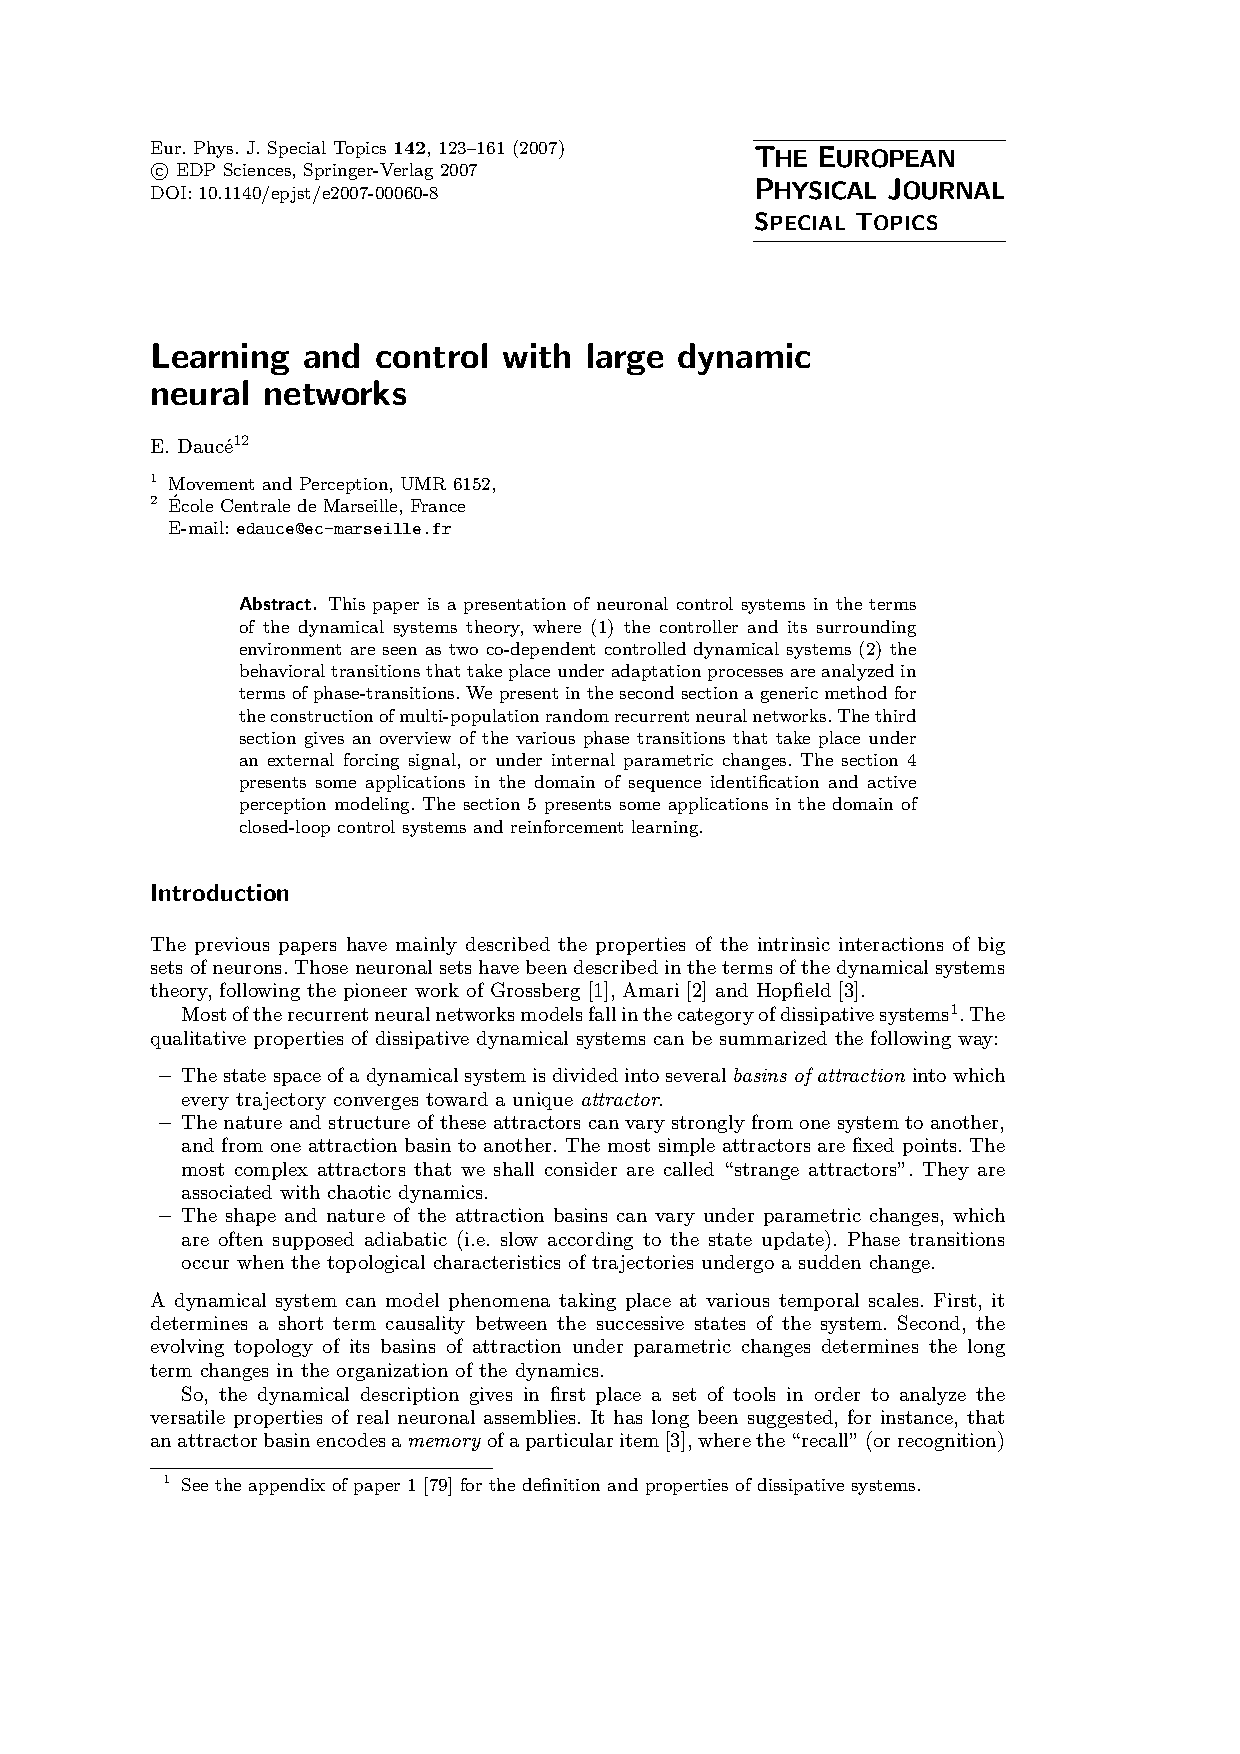
\includepdf[pages=1-10]{pdf/epj-st-2007.pdf}
%\end{minipage}
%}
% Histoires
\section{Modèles pour la perception spatio-temporelle}

% un point important : la prise en compte des delais!!! conditionne l'anticipation sensorielle, la synchronisation agent-environnement, l'apprentissage de séquences.

% perception et non-sens

% L'idée de Freeman. L'enregistrement multi-électrodes. Potentialité et instanciation (choix d'une orbite). 

Karl Friston : ce qui est perçu est principalement l'ecart à la prediction (predictive coding).  Dynamical Causal modelling.
``Modern reformulations suggest
that both inference on states (that is, perception) and
inference on parameters (that is, learning) minimize
free energy (that is, minimize prediction error) and
serve to bound surprising exchanges with the world.'' (Friston, 2010)

et aussi ``rewards correspond to innate priors that constrain policies.''


% D'apres le mecanisme de Hopfield, la memoire est principalement un mecanisme d'interpolation

% Le point de vue informationnel : 

\subsection{Substrat - codage topographique}

% Re

Mean field

Field computation

Expressivité discrète - continue

La structure (ou l'expressivité) du substrat conditionne/caractérise la manière dont l'environnement est perçu (attention raisonnemnt qui se mord la queue). 
Par exemple, l'existence d'un procesus de pattern matching avec seuil conditionne la perception du monde sous forme de transitions brusques et de relaxations
vers des attracteurs.
L'existence d'un modèle linéaire conditionne la perception du monde sous la forme de reponse linéaire (asservissement) à l'erreur de prédiction.
L'existence de delais conditionne la perception des causalités temporelles. 



\subsection{Bruit et choix}

% Modèlmes RL - Actor--critic
L'activité intrinsèque (non necessairement bruit). ``sculpte'' la reponse comportementale par des phénomènes de résonance.  
Bruit destructeur / bruit createur. Darwinisme. On peut voir le bruit d'etat comme un facteur perturbateur de couplage. 


Rappels sur les 2 approches synthétisees dans EPJST : supervisé et renforcement.

L'apprentissage par renforcement apporte une notion nouvelle : bruit générateur (créateur). ``création d'information'' : ``enact'' (promulguer) 
création de faits nouveaux (orientations nouvelles, deplacements nouveaux, emplois nouveaux). ``Angle mort'' des sciences cognitives. 
Contingence et capture. 
Il est important de distinguer l'approche ``pattern matching'' qui repose sur une capture passive des regularites statistiques et l'approche RL qui à la fois capture 
et genere les patterns.
Conceptuellement problematique du point de vue de la theorie de l'information (notion d'emetteur et de recepteur brouillées), sauf peut-etre du point de vue global (inobservé)
auquel cas il n'y a ni emetteur ni recepteur.

On peut assimiler un fait à un couple (perception, action).

Et bien sûr approche énactive : on ne perçoit que ce sur quoi on peut agir. 
"Le monde (visuel) est (quelque chose qui est) constitué par l'action" (Varela)

La théorie du renforcement a tendance à définir l'activité comme reflétant la valeur de la situation (du couple (s,a)).
Dans ce cadre, l'état du système n'est pas une représentation du monde exterieur mais plutot une batterie de ``notes'' attribuées
aux différentes réponses motrices potentielles étant donnée la situation .

% L'état central fluctuant est popularisé par J-D Vincent


Les variables de contrôle (rewards) arrivent par d'autres canaux. 

\subsection{Plasticité séquentielle}

% STDP
% Image du papillon-chenille

\section{Mouvements}
% continuous RL

\section{Carte et Territoire}
% MAPS

\section{Multistabilités}
% DTI

\section{}


\chapter{Projet scientifique}

\section{Le radeau des cîmes}


\chapter{Conclusion}

\chapter*{Annexes}

\end{document}
